%%%%%%%%%%%%%%%%%%%%%%%%%%%%%%%%%%%%%%%%%%%%%%
\section{Beam plug}
\label{sec:beamplug}

\fixme{structure of section needs fixing}

In order to allow the particle beam to enter the active TPC region with minimal energy loss and multiple scattering from upstream materials, a beam window penetration is inserted into the cryostat insulation layers (described in Section~\ref{subsec:beamwindow}). An additional inner 
beam plug will be installed inside the cryostat to allow the particle beam to enter the active TPC volume without having to pass through 
a $\approx$45~cm thick passive LAr layer and the field cage.




The beam plug is designed to displace the passive LAr layer between the TPC field cage and the inner cryostat membrane. As illustrated in Figure~\ref{fig:beamplug}, it is a cylidrical glass-fiber composite pressure vessel about 50cm in length and  22cm in diameter. It is filled with dry nitrogen gas via a stainless steel line that extends to the top of the cryostat. The pressure inside the beam plug is maintained externally up to 25 psi from room to LAr temperatures. A pressure relief valve (or burst disk) will be installed on the nitrogen fill line on the top of the cryostat (externally) to ensure the pressure inside the beam plug does not exceed the safety level. The component-level view of the beam plug is shown in Figure~\ref{fig:beamplug_components}.  The beam plug is secured to the field cage support structure as described in Section~\ref{subsec:fc-beamplug}. The front portion of the beam plug extends 5~cm beyond the profiles to inside the active region of the TPC through an opening on the field cage. The field cage support is designed with sufficient strength and stiffness to support the weight of the beam plug while it is suspended in air. 
When the cryostat is filled with LAr, the beam plug is roughly neutrally buoyant.  The total internal volume of the beam plug is about 16 liters. 

The requirements on the acceptable leak rate is between $7.8\times 10^{-5}$ scc/s to $15.6\times 10^{-5}$ scc/s. This is a very conservative leak rate and is roughly equivalent to 15\% of the nitrogen in the beam plug leaked over a period of a year.
  In a worst case scenario with all the nitrogen in the beam plug leaking into the LAr cryostat, the increase in concentration is about 0.1 ppm, which is still a factor of 10 below the acceptable level as specified by light detection requirements.
  \fixme{need some reference with details for this requirement}
  At nominal operation, the voltage difference across the beam plug (between the first and the last grading ring) is 165kV. 
  To minimize risk of electrical discharges, the beam plug is divided into sections and each section is bonded to stainless steel conductive grading rings. The grading rings are connected in series with two parallel path of resistor chains. There are 7 grading rings. The ring that is closest to the field cage is electrically connected to one of the field cage profiles. 
  The last ring near the cryostat wall is grounded to the stainless steel membrane via a short grounding cable. 
  The type and value of the resistor is still under evaluation. A likely candidate is the high voltage Super Mox 15G$\Omega$ resistor by OHMITE. The maximum total power dissipated by the resistor chain is about 0.6W.


\begin{cdrfigure}[Beam plug]{beamplug}{The beam plug is a  composite pressure vessel filled with dry nitrogen gas. The vessel is about 50cm in length and about 22cm in diameter. The pressure vessel is divided into sections with each section bonded to a stainless steel grading ring. The grading rings are connected by two parallel paths of resistor chain.}
  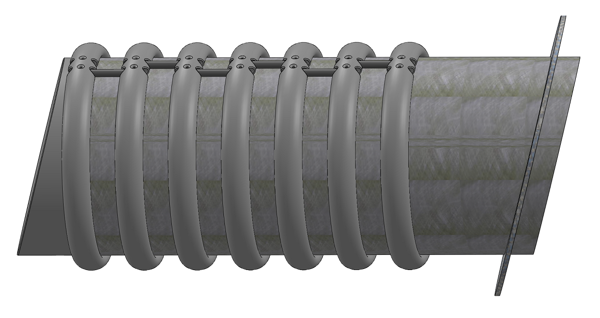
\includegraphics[width=0.75\textwidth]{beamplug.png}
\end{cdrfigure}

\begin{cdrfigure}[Beam plug component-level view]{beamplug_components}{Component-level view of the beam plug showing alternating electrode and composite ring structure.}
  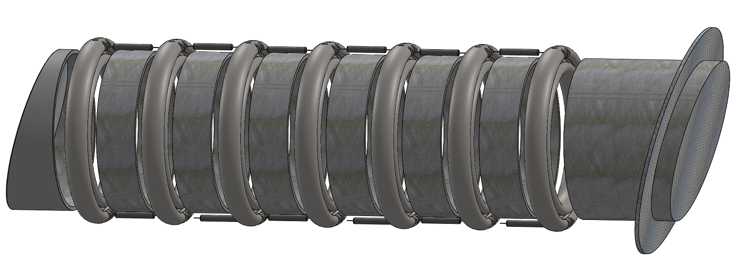
\includegraphics[width=0.85\textwidth]{beamplug_components.png}
\end{cdrfigure}

The metal electrode rings are spaced at regular intervals and interspersed with composite tube sections. The shape of the rings has been designed to minimize high electric field corners. The results of the field calculations are shown in Figures~\ref{fig:beamplug_ring1} and~\ref{fig:beamplug_ring2}. The average field in the vicinity of the beam plug is about 4.4 kV/cm. The maximum field of 15.7 kV/cm is on the electrode ring surface. In all regions the field is well below the 30 kV/cm limit.
\fixme{citation to doc describing limit would be good}

\begin{cdrfigure}[Beam plug electrodes]{beamplug_ring1}{Electric field calculation of the electrode ring design. The average field in the beam plug region is about 4.4 kV/cm. The maximum field of 15.7 kV/cm is on the electrode ring surface. }
  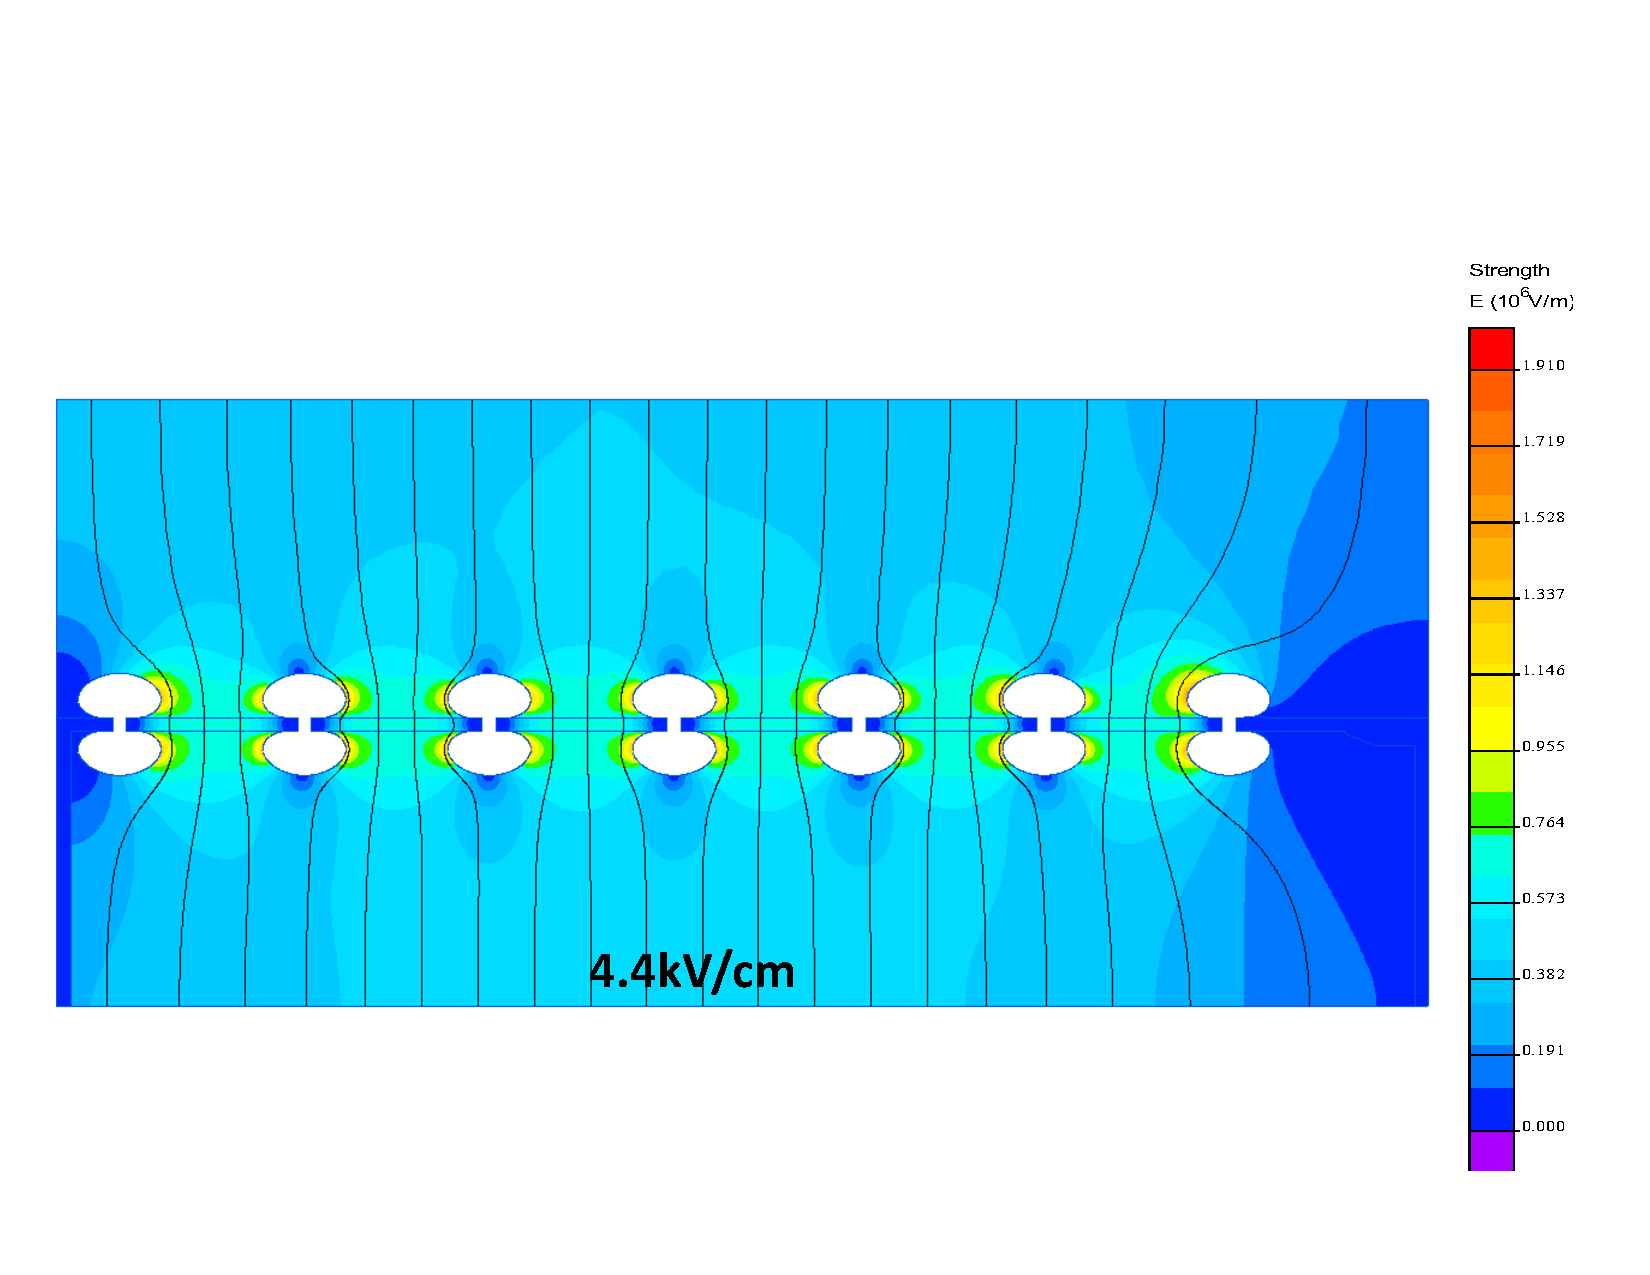
\includegraphics[width=0.85\textwidth]{beamplug_ring1.pdf}
\end{cdrfigure}

\begin{cdrfigure}[Beam plug electrode]{beamplug_ring2}{Electric field calculation near the vicinity of the electrode. The shape of the ring minimizes the high field region near the joints between the electrode, LAr, and composite shell. The field is well below the 30 kV/cm limit in all regions.}
  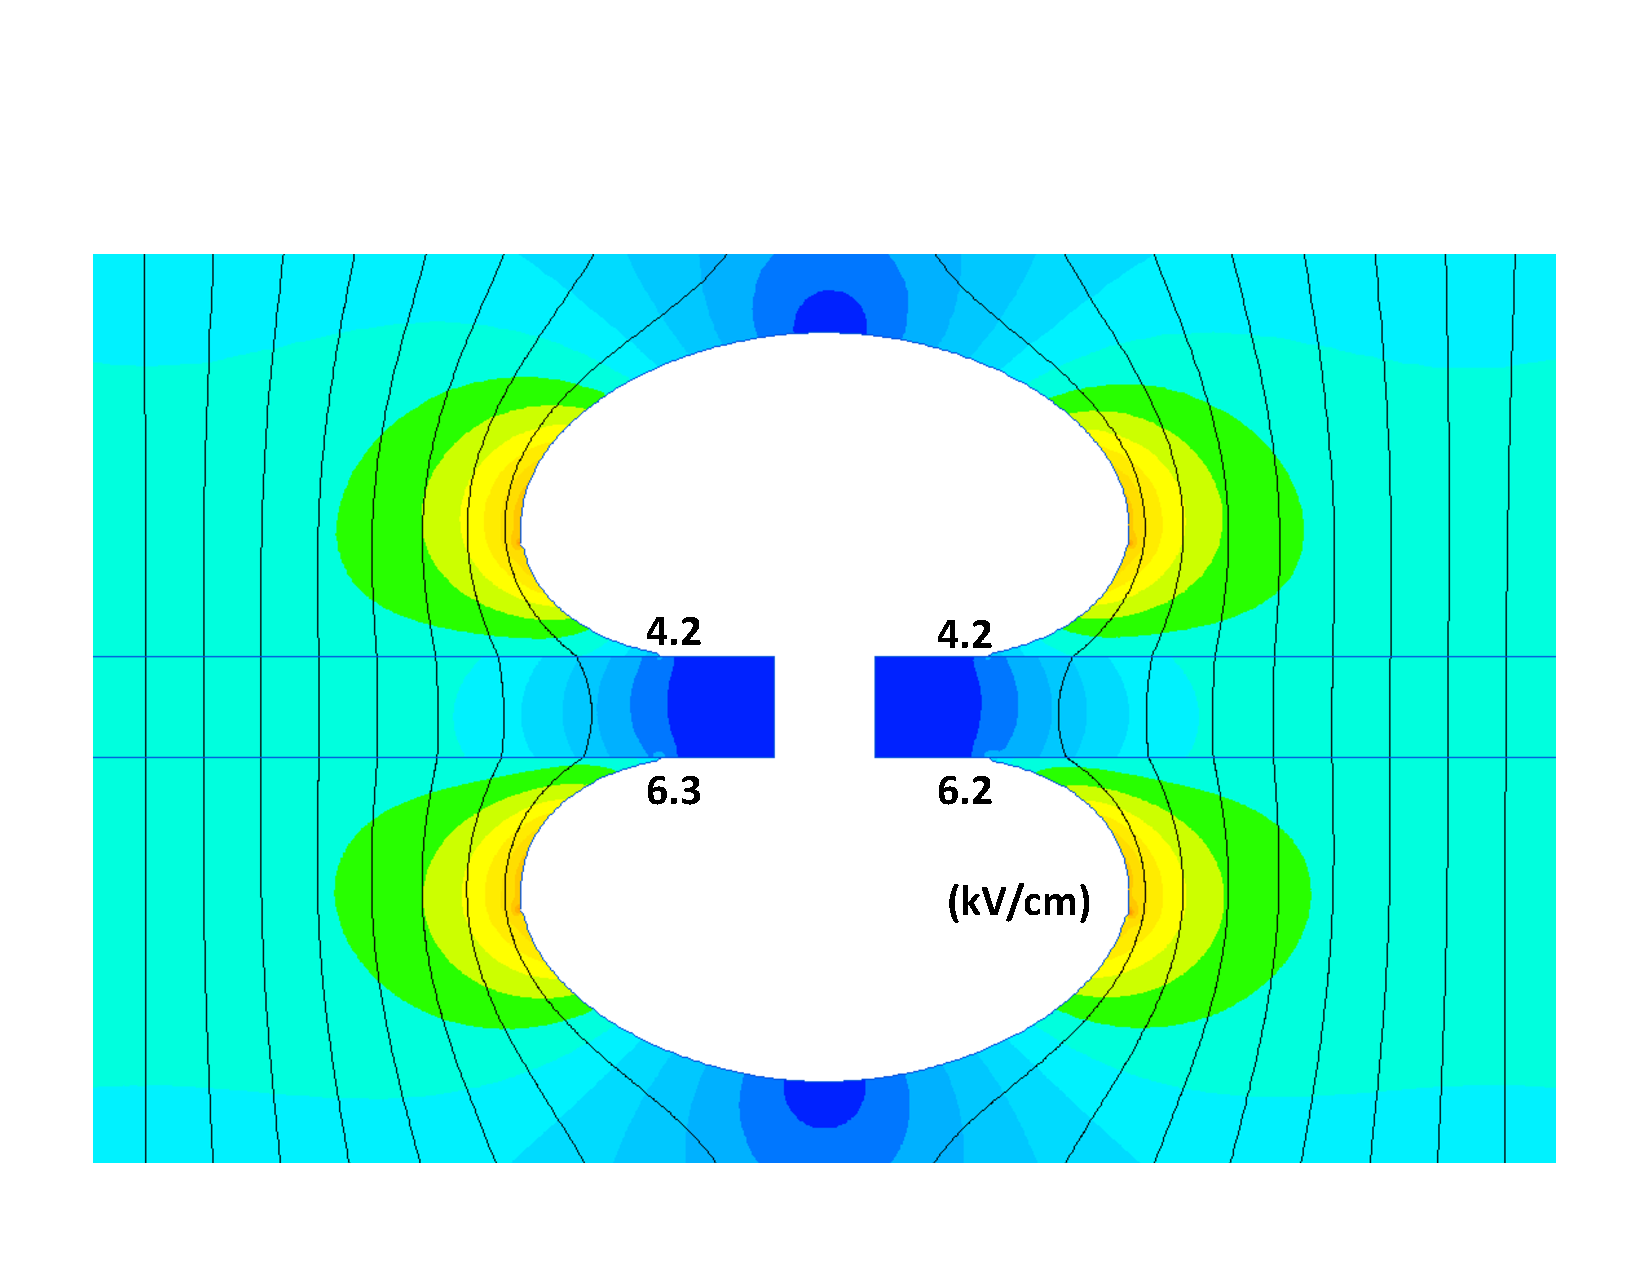
\includegraphics[width=0.5\textwidth]{beamplug_ring2.pdf}
\end{cdrfigure}

A summary of the beam plug requirements and parameters list are given in Table~\ref{tab:bprequirements}.

\begin{cdrtable}[Beam plug requirements]{lll}{bprequirements}{Beam plug requirements and parameters list}
Parameter & Value & Notes \\ \toprowrule
Dimensions & & Defined by CAD model \\ 
~~Internal Diameter (est) & 200~mm & At composite ring ID surface; \\
                          &        & tolerance for assembly \\ 
~~Wall thickness (est) & 8~mm & Tolerance for assembly \\ 
~~Length (est) & 495~mm $\pm$ 1~mm & Overall (Normal Distance) \\ 
               & 577~mm $\pm$ 1~mm & Overall (Absolute Distance) \\ \colhline 
Metal End Cap Angle & (16.2$\pm$0.25)$^\circ$ & From perpendicular; \\ 
                    &                         &maintain length tolerance \\ 
Composite End Cap   & (16.2$\pm$0.5)$^\circ$ & From perpendicular; \\ 
                    &                        & maintain length tolerance \\ 
Flange Angle        & (16.2$\pm$0.25)$^\circ$ & From perpendicular \\ \colhline 
Tolerances  & ASME Y14.5 2009 & Where useful to convey design intent \\
            &                 & and function \\ 
Materials used   & & Electrically insulating; selected from or\\
                 & & approved per FNAL LAr purity list \\ 
Epoxy system & Hysol 9309.2 NA & Rated for cryogenic use\\
Electrode Rings & 304 Stainless steel & \\ \colhline 
Resistor Type & OHMITE Super-Mox 930 Series & \\
Resistor Value & 15~G$\Omega$ & \\
Number of resistors & 6 & \\
Power dissipation &  &\\ 
~~Per resistor    & $\approx$0.1W & \\
~~Total           & $\approx$0.6W & \\ \colhline 
Operating Voltage & Up to 180 kV end-to-end &  \\ 
Operating Temperature & 25$^\circ$~C & Room temperature \\ 
                      & -185$^\circ$~C & LAr temperature \\ 
Operating Pressure    & 25~psi & MAWP at operating temperature \\ \colhline
Pressure Environment & 14.7 psi & Ambient temperature \\
(External)           & 19.9 psi & LAr temperature \\ \colhline
Internal Volume & 15.5 liter (est.) & Internal \\
                & 22 liter (est.) & External displacement \\ \colhline
Permeability/Leak Rate  & 7.8$\times$10$^{-5}$ scc/s to & Total volumetric, $N_2$ gas \\
Range                             & 15.6$\times$10$^{-5}$ scc/s & He gas equivalent\\ \colhline
Operating Lifetime   & 1 yr  &  \\
Lifetime Operational Thermal & 4 & \\
~Cycles to 77 K & & \\ \colhline
Shock Loading & & No design shock loading \\
Vibration Loading & & No design vibration loading \\ \colhline
Flange Profile & & Geometry per LBNL ICD \\
Weight (est.) & 75 lb [34 kg] & With SS304 electrode rings \\
Buoyancy Load (est.) & 67.5 lb [31 kg] & \\
Pressure Port & & Ground cap interface per LBNL \\ \colhline
Design Safety Factor & 2 & On MAWP (=50 psi) \\
Pressure Test Factor & 1.5 & Pneumatic test \\
High Voltage Tests & (180 kV equivalent) & \\ 
\end{cdrtable}



\subsection{Field cage resistor divider chain with beam plug}
The resistor divider chain of the beam plug is tied to the main field cage profile. To maintain the 3 kV voltage drop across all field cage profiles, a second resistor divider board is added in parallel to the nominal board for the first 5 field cage profiles closest to the CPA. This modification is only needed for the field cage panel with the beam plug attached. The circuit diagram for the proposed scheme and the resistor values are shown in Figure~\ref{fig:beamplug_resistordivider}.
\begin{cdrfigure}[Beam plug resistor divider chain]{beamplug_resistordivider}{The resistor divider circuit for the end-wall field cage panel with the beam plug. The proposed resistor values for the main, parallel divider boards, and the beam plug are given in the tables.}
  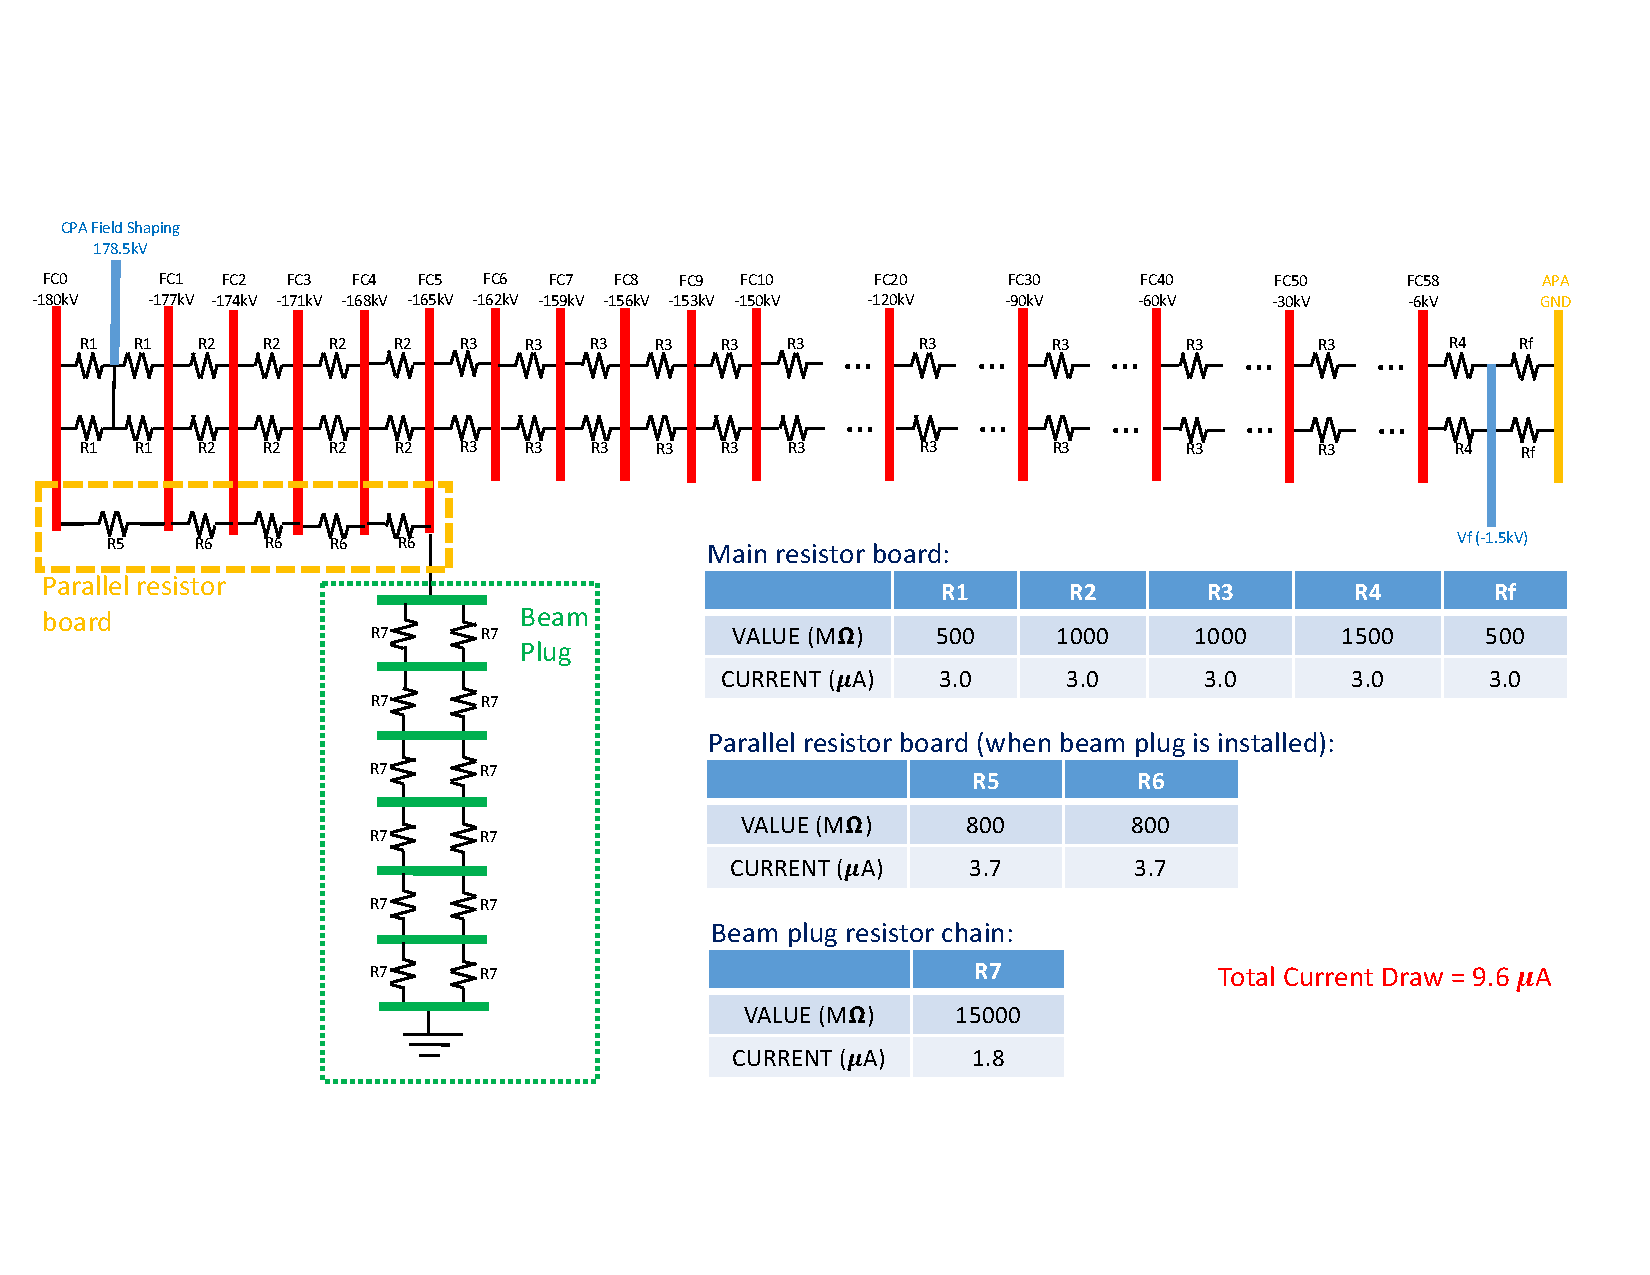
\includegraphics[width=0.85\textwidth]{beamplug_resistordivider.pdf}
\end{cdrfigure}




